\documentclass[11pt,a4paper]{article}

\usepackage[T1]{fontenc}
\usepackage[utf8]{inputenc}
\usepackage{lmodern}
\usepackage[english]{babel}

\usepackage{amsmath,amssymb,amsthm}
\usepackage{booktabs}
\usepackage{graphicx}
\usepackage{float}
\usepackage[a4paper,margin=1in]{geometry}
\usepackage{hyperref}
\usepackage{tikz}
\usetikzlibrary{arrows.meta,decorations.pathreplacing}
\usepackage{xcolor}
\usepackage{microtype}
\setlength{\parindent}{0pt}
\setlength{\parskip}{0.5em}

\title{Continuation vs Reversal After Extreme Short-Term SPY Moves: Sensitivity to Target Construction}
\author{Christian Lauterbach}
\date{\today}

\begin{document}
	
	\maketitle
	\tableofcontents
	\newpage
	
	\section{Introduction}
	
	The object of interest in this paper is the short-horizon price response following an extreme intraday move. Conditional on the detection of such an event at time \(t\), the relevant question is whether the subsequent path is more likely to exhibit continuation or reversal. With \(X_t\) denoting a vector of pre-event features and \(Y_t \in \{0,1\}\) a continuation-versus-reversal label, the predictive problem is whether the conditional law
	\[
	\mathbb{P}(Y_t = y \mid X_t), \qquad y \in \{0,1\},
	\]
	depends nontrivially on \(X_t\).
	
	A central methodological complication is that \(Y_t\) is not primitive. Rather, it is induced by a rule imposed on the post-event path. Consequently, the learning problem is itself target-dependent. Even with the raw price process, the event-detection rule, and the pre-event feature set held fixed, a change in the label construction changes the effective sample
	\[
	\{(X_t,Y_t)\}_{t \in \mathcal{T}_{\mathrm{event}}},
	\]
	and thereby may alter the number of admissible events, the class proportions, the time-to-resolution distribution, and the measured out-of-sample performance.
	
	The paper studies this dependence under a common event-detection backbone. Two target constructions are compared. In Method I, continuation and reversal are defined relative to the direction of the extreme event itself. In Method II, the reference direction is defined only after a short post-event interval, so that the label is indexed to the immediate post-event move rather than to the original event direction. Thus, the comparison is not merely terminological; it isolates the effect of redefining the directional reference while leaving the detection rule and feature map unchanged.
	
	This distinction has two statistical consequences. First, the delayed reference used in Method II can induce a stronger marginal continuation bias by conditioning, albeit implicitly, on a short confirmation step. Second, that same delay introduces temporal separation between the feature vector \(X_t\) and the effective anchor of the label. Hence a target may become more directionally biased in an unconditional sense while becoming less predictable from pre-event information in a conditional sense. Put differently, a stronger base-rate asymmetry need not imply greater feature-based learnability.
	
	The empirical results are consistent with this interpretation. Relative to Method I, Method II produces a more asymmetric label distribution in favor of continuation, yet exhibits weaker evidence of conditional predictability from the common pre-event feature set. Method I, by contrast, displays a weaker marginal continuation tendency but stronger discrimination beyond the corresponding majority baseline. This suggests a bias--learnability tradeoff: waiting to confirm direction may strengthen unconditional directional structure while attenuating the relevance of information available at the event time.
	
	The contribution of the paper is therefore comparative rather than prescriptive. The aim is not to assert a robust tradable signal, but to show that under a fixed event-detection architecture and a common pre-event feature set, the apparent predictability of continuation versus reversal is materially sensitive to target construction. In particular, redefining the reference direction changes not only the semantics of the label, but also its marginal distribution and its conditional relation to \(X_t\).
	
	\section{Data and Event Construction}
	
	\subsection{Data Source and Sampling Frequency}
	
	Let \(S_t\) denote the SPY price observed on a \(2\)-minute grid. The empirical analysis uses intraday SPY data downloaded from \texttt{yfinance}. Since Yahoo Finance provides only a limited recent history for \(2\)-minute bars, the available sample is restricted to approximately the most recent \(60\) calendar days. The study should therefore be interpreted as a short-sample exploratory analysis rather than a large-sample estimate of a stable market effect.
	
	The design is event-driven rather than bar-driven. Thus the basic statistical unit is not an arbitrary \(2\)-minute bar, but an identified extreme-move event. Only such event times enter the final dataset.
	
	\subsection{Feature Construction}
	
	For each time \(t\), define the one-bar return
	\[
	r_t^{(1)} = \frac{S_t}{S_{t-1}} - 1
	\]
	and the \(k\)-bar event return
	\[
	r_t^{(k)} = \frac{S_t}{S_{t-k}} - 1.
	\]
	These quantities are used to construct both the event-detection rule and the pre-event feature vector.
	
	The feature set is restricted to information available at or before the event time \(t\). This is particularly important for Method II, in which the label reference direction is determined only after the short interval \([t,t+h_0]\). It includes return-based, volatility-based, volume-based, and candlestick-style features, such as
	\[
	r_t^{(k)},\quad \sigma_t^{(k)},\quad z_t,\quad \text{volume ratios},\quad \text{short-lag returns},\quad \text{rolling return moments},
	\]
	together with measures of intrabar shape and time-from-open. No post-event variables are used as model inputs.
	
	Formally, each retained event contributes an observation of the form
	\[
	(X_t,Y_t),\qquad t \in \mathcal{T}_{\mathrm{event}},
	\]
	where \(X_t\) is the pre-event feature vector and \(Y_t \in \{0,1\}\) is assigned by one of the target-construction rules described in the next section.
	
	\subsection{Shared Event-Detection Rule}
	
	The event-detection backbone is identical across both methods. First compute the \(k\)-bar return
	\[
	r_t^{(k)} = \frac{S_t}{S_{t-k}} - 1.
	\]
	Next define a rolling volatility proxy over a lookback window of length \(m\):
	\[
	\sigma_t^{(m)} = \operatorname{sd}\!\left(r_{t-m+1}^{(k)},\dots,r_t^{(k)}\right),
	\]
	and the standardized event score
	\[
	z_t = \frac{|r_t^{(k)}|}{\sigma_t^{(m)}}.
	\]
	An event is declared whenever
	\[
	z_t \ge z.
	\]
	
	In the empirical implementation, the common event-detection parameters are
	\[
	k=3,\qquad m=15,\qquad z=2.
	\]
	Hence an event corresponds to a sufficiently large \(3\)-bar return relative to a local \(15\)-bar volatility scale.
	
	\subsection{Cooldown Rule and Event Set}
	
	To avoid dense clusters of highly overlapping detections, a cooldown rule is imposed. If an event is recorded at time \(t\), then any further candidate events within the next prescribed number of bars are ignored. This ensures that the final sample consists of separated extreme-move episodes rather than multiple near-duplicate detections from the same local burst of volatility.
	
	Let \(\mathcal{T}_{\mathrm{event}}\) denote the retained event times after this filtering step. In the empirical implementation, the cooldown parameter is
	\[
	\text{cooldown}=10.
	\]
	Thus at least \(10\) bars must separate consecutive retained events.
	
	\subsection{Post-Event Horizon and Sample Retention}
	
	Conditional on an event at time \(t\), the post-event path is examined over a finite horizon
	\[
	j = 1,\ldots,h_{\max}.
	\]
	Events too close to the end of the sample are dropped if the required post-event horizon is not available. In the empirical implementation,
	\[
	h_0 = 1, \qquad h_{\max} = 30,
	\]
	where \(h_0\) is the short post-event reference interval used in Method II, and \(h_{\max}\) is the maximum number of bars over which the event is allowed to resolve.
	
	The role of \(h_0\) is conceptually important. In Method I, the reference direction is fixed at the event time \(t\), so the target is anchored directly to the detected extreme move. In Method II, the reference direction is fixed only after the interval \([t,t+h_0]\). Thus Method II introduces a short temporal gap between the pre-event feature vector \(X_t\) and the effective reference point used to define the label. This distinction is central to the later comparison.
	
	\section{Label Definitions}
	
	Conditional on an event having been detected at time \(t\), the label \(Y_t \in \{0,1\}\) is assigned by one of two alternative rules. The event-detection backbone is identical across both methods; only the target construction differs.
	
	
	\subsection{Method I: Event-Direction Reference}
	
	In the first specification, the direction of the extreme move itself is used as the reference direction. Define
	\[
	\operatorname{event\_sign}_t = \operatorname{sign}\!\left(r_t^{(k)}\right),
	\qquad
	\operatorname{event\_size}_t = \left|r_t^{(k)}\right|.
	\]
	From the event price \(S_t\), define the symmetric barrier levels
	\[
	S_t^{+} = S_t\bigl(1+\alpha \lvert r_t^{(k)}\rvert\bigr),
	\qquad
	S_t^{-} = S_t\bigl(1-\alpha \lvert r_t^{(k)}\rvert\bigr).
	\]
	The post-event path is then examined over
	\[
	j=1,\dots,h_{\max}.
	\]
	
	If the event is upward, i.e.
	\[
	\operatorname{event\_sign}_t=+1,
	\]
	then continuation means that the upper barrier is hit first, while reversal means that the lower barrier is hit first:
	\[
	Y_t =
	\begin{cases}
		1, & \text{if } S_{t+j} \text{ first reaches } S_t^{+},\\[1mm]
		0, & \text{if } S_{t+j} \text{ first reaches } S_t^{-}.
	\end{cases}
	\]
	
	If the event is downward, i.e.
	\[
	\operatorname{event\_sign}_t=-1,
	\]
	the interpretation is reversed:
	\[
	Y_t =
	\begin{cases}
		1, & \text{if } S_{t+j} \text{ first reaches } S_t^{-},\\[1mm]
		0, & \text{if } S_{t+j} \text{ first reaches } S_t^{+}.
	\end{cases}
	\]
	
	Equivalently, Method I defines
	\[
	Y_t=1 \iff \text{the first barrier hit lies in the direction of the original event,}
	\]
	\[
	Y_t=0 \iff \text{the first barrier hit lies opposite to the original event.}
	\]
	
	If neither barrier is reached by \(h_{\max}\), the event is treated as unresolved and excluded.
	

% in the document
\begin{figure}[H]
	\centering
	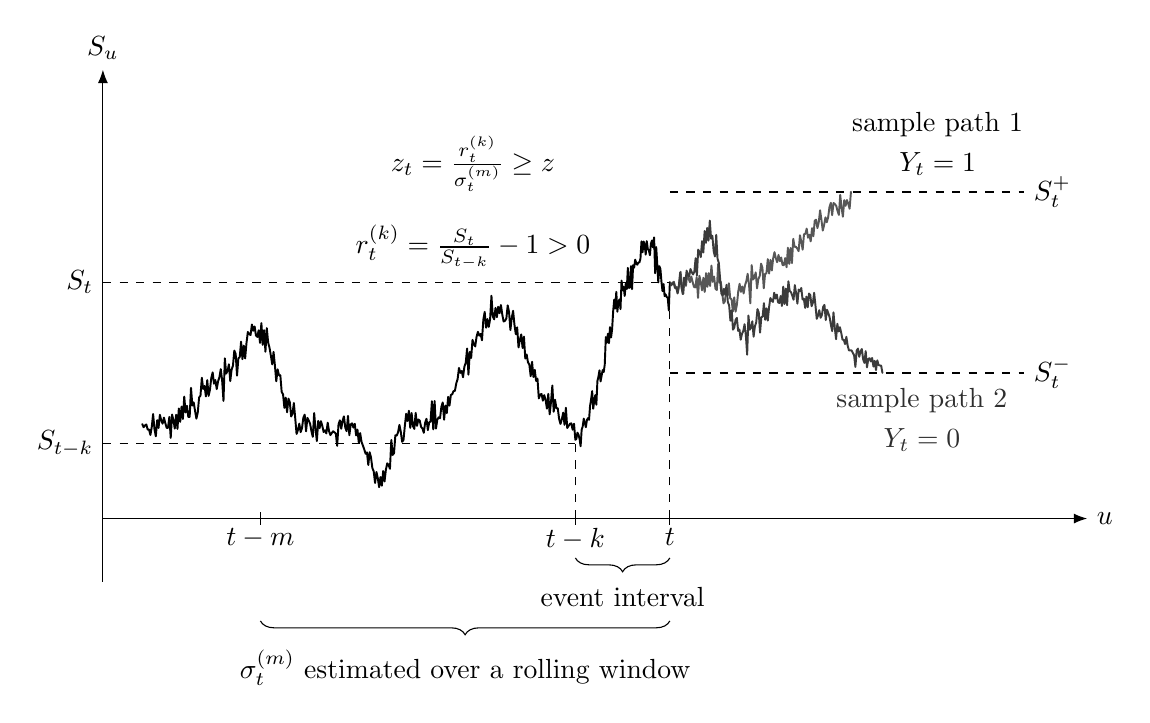
\begin{tikzpicture}[x=1cm,y=1cm,>=Latex]
		
		% key times
		\coordinate (tm) at (2.0,0);
		\coordinate (tk) at (6.0,0);
		\coordinate (t)  at (7.2,0);
		
		% axes
		\draw[->] (0,0) -- (12.5,0) node[right] {$u$};
		\draw[->] (0,-0.8) -- (0,5.7) node[above] {$S_u$};
		
		
		
	% ---------- Brownian-looking pre-event path with 4 tweakable pulls ----------
	\pgfmathsetseed{9}
	
	\def\graycoords{}
	
	\pgfmathsetmacro{\xA}{0.5}
	\pgfmathsetmacro{\xMid}{6.25}
	\pgfmathsetmacro{\xB}{7.2}
	
	\pgfmathsetmacro{\yA}{1.2}
	\pgfmathsetmacro{\yB}{3.00}
	
	\pgfmathsetmacro{\xTk}{6.0}
	\pgfmathsetmacro{\yTk}{1}
	
	\pgfmathtruncatemacro{\None}{320}
	\pgfmathtruncatemacro{\Ntwo}{90}   % more points on [t-k,t]
	
	% extra pulls on the event interval [t-k, t]
	\pgfmathsetmacro{\cEventOne}{6.45}
	\pgfmathsetmacro{\aEventOne}{28}
	\pgfmathsetmacro{\wEventOne}{0.25}
	
	\pgfmathsetmacro{\cEventTwo}{6.82}
	\pgfmathsetmacro{\aEventTwo}{21}
	\pgfmathsetmacro{\wEventTwo}{0.34}
	
	% =========================================================
	% 4 pulls to shape the path
	% =========================================================
	\pgfmathsetmacro{\cOne}{1.5}
	\pgfmathsetmacro{\aOne}{8}
	\pgfmathsetmacro{\wOne}{0.4}
	
	\pgfmathsetmacro{\cTwo}{2}
	\pgfmathsetmacro{\aTwo}{15}
	\pgfmathsetmacro{\wTwo}{0.3}
	
	\pgfmathsetmacro{\cThree}{3.5}
	\pgfmathsetmacro{\aThree}{-10}
	\pgfmathsetmacro{\wThree}{0.2}
	
	\pgfmathsetmacro{\cFour}{5}
	\pgfmathsetmacro{\aFour}{21}
	\pgfmathsetmacro{\wFour}{0.5}
	
	% extra controls
	\pgfmathsetmacro{\noiseLevel}{0.1}
	\pgfmathsetmacro{\pullLevel}{0.070}
	\pgfmathsetmacro{\baseLevel}{1.00}
	
	% ---------- Part 1: random walk + 4 broad pulls on [xA, xTk] ----------
	\pgfmathsetmacro{\y}{\yA}
	\xdef\graycoords{(\xA,\yA)}
	
	\foreach \i in {1,...,\None}{
		\pgfmathsetmacro{\x}{\xA + (\xTk-\xA)*\i/\None}
		\pgfmathsetmacro{\xi}{rnd+rnd+rnd+rnd+rnd+rnd+rnd+rnd+rnd+rnd+rnd+rnd-6}
		
		\pgfmathsetmacro{\shape}{
			\baseLevel
			+ \aOne   * exp(-((\x-\cOne)^2)   / (\wOne*\wOne))
			+ \aTwo   * exp(-((\x-\cTwo)^2)   / (\wTwo*\wTwo))
			+ \aThree * exp(-((\x-\cThree)^2) / (\wThree*\wThree))
			+ \aFour  * exp(-((\x-\cFour)^2)  / (\wFour*\wFour))
		}
		
		\pgfmathsetmacro{\y}{\y + \noiseLevel*\xi + \pullLevel*(\shape-\y)}
		
		\ifnum\i=\None
		\pgfmathsetmacro{\y}{\yTk}
		\fi
		
		\xdef\graycoords{\graycoords (\x,\y)}
	}
	
	% ---------- Part 2: from (xTk,yTk) to (xB,yB) ----------
	\pgfmathsetmacro{\y}{\yTk}
	\pgfmathsetmacro{\tauMid}{(\xMid-\xTk)/(\xB-\xTk)}
	
	\foreach \i in {1,...,\Ntwo}{
		\pgfmathsetmacro{\tau}{\i/\Ntwo}
		\pgfmathsetmacro{\x}{\xTk + (\xB-\xTk)*\tau}
		\pgfmathsetmacro{\xi}{rnd+rnd+rnd+rnd+rnd+rnd+rnd+rnd+rnd+rnd+rnd+rnd-6}
		
		\pgfmathsetmacro{\theta}{max(0,(\tau-\tauMid)/(1-\tauMid))}
		
		\pgfmathsetmacro{\target}{
			\yTk
			+ (\yB-\yTk)*(\theta^1.8)
			+ \aEventOne * exp(-((\x-\cEventOne)^2)/(\wEventOne*\wEventOne))
			+ \aEventTwo * exp(-((\x-\cEventTwo)^2)/(\wEventTwo*\wEventTwo))
		}
		
		% more jaggedness, less deterministic pull
		\pgfmathsetmacro{\noise}{0.12 - 0.03*\theta}
		\pgfmathsetmacro{\pull}{0.035 + 0.16*\theta^2}
		
		\pgfmathsetmacro{\y}{\y + \noise*\xi + \pull*(\target-\y)}
		
		\ifnum\i=\Ntwo
		\pgfmathsetmacro{\y}{\yB}
		\fi
		
		\xdef\graycoords{\graycoords (\x,\y)}
	}
	
	\draw[line width=0.7pt, line join=round, line cap=round]
	plot coordinates {\graycoords};
	
	% ---------- Pink path ----------
	\pgfmathsetseed{9}
	
	\def\pinkcoords{}
	
	\pgfmathsetmacro{\xPzero}{\xB}
	\pgfmathsetmacro{\xPone}{9.5}
	
	\pgfmathsetmacro{\yPzero}{\yB}
	\pgfmathsetmacro{\yPone}{4.15}
	
	\pgfmathtruncatemacro{\NPink}{135}
	
	% tweak these
	\pgfmathsetmacro{\cPinkOne}{8}
	\pgfmathsetmacro{\aPinkOne}{-8}
	\pgfmathsetmacro{\wPinkOne}{0.1}
	
	\pgfmathsetmacro{\cPinkTwo}{8.5}
	\pgfmathsetmacro{\aPinkTwo}{2}
	\pgfmathsetmacro{\wPinkTwo}{0.05}
	
	\pgfmathsetmacro{\cPinkThree}{9.2}
	\pgfmathsetmacro{\aPinkThree}{5.8}
	\pgfmathsetmacro{\wPinkThree}{0.67}
	
	\pgfmathsetmacro{\noisePink}{0.1}
	\pgfmathsetmacro{\pullPink}{0.15}
	
	\pgfmathsetmacro{\y}{\yPzero}
	\xdef\pinkcoords{(\xPzero,\yPzero)}
	
	\foreach \i in {1,...,\NPink}{
		\pgfmathsetmacro{\tau}{\i/\NPink}
		\pgfmathsetmacro{\x}{\xPzero + (\xPone-\xPzero)*\tau}
		\pgfmathsetmacro{\xi}{rnd+rnd+rnd+rnd+rnd+rnd+rnd+rnd+rnd+rnd+rnd+rnd-6}
		
		\pgfmathsetmacro{\target}{
			\yPzero + (\yPone-\yPzero)*(\tau^2.0)
			+ \aPinkOne   * exp(-((\x-\cPinkOne)^2)   / (\wPinkOne*\wPinkOne))
			+ \aPinkTwo   * exp(-((\x-\cPinkTwo)^2)   / (\wPinkTwo*\wPinkTwo))
			+ \aPinkThree * exp(-((\x-\cPinkThree)^2) / (\wPinkThree*\wPinkThree))
		}
		
		\pgfmathsetmacro{\noise}{\noisePink - 0.02*\tau}
		\pgfmathsetmacro{\pull}{0.02 + \pullPink*\tau^2}
		
		\pgfmathsetmacro{\y}{\y + \noise*\xi + \pull*(\target-\y)}
		
		\ifnum\i=\NPink
		\pgfmathsetmacro{\y}{\yPone}
		\fi
		
		\xdef\pinkcoords{\pinkcoords (\x,\y)}
	}
	
	\draw[black!66, line width = 0.7pt, line join=round, line cap=round]
	plot coordinates {\pinkcoords};
	
	% ---------- Green path ----------
	\pgfmathsetseed{9}
	
	\def\greencoords{}
	
	\pgfmathsetmacro{\xGzero}{\xB}
	\pgfmathsetmacro{\xGone}{9.9}
	
	\pgfmathsetmacro{\yGzero}{\yB}
	\pgfmathsetmacro{\yGone}{1.85}
	
	\pgfmathtruncatemacro{\NGreen}{165}
	
	% tweak these
	\pgfmathsetmacro{\cGreenOne}{7.7}
	\pgfmathsetmacro{\aGreenOne}{28}
	\pgfmathsetmacro{\wGreenOne}{0.2}
	
	\pgfmathsetmacro{\cGreenTwo}{8}
	\pgfmathsetmacro{\aGreenTwo}{-15}
	\pgfmathsetmacro{\wGreenTwo}{0.43}
	
	\pgfmathsetmacro{\cGreenThree}{9.68}
	\pgfmathsetmacro{\aGreenThree}{-4.8}
	\pgfmathsetmacro{\wGreenThree}{0.65}
	
	\pgfmathsetmacro{\noiseGreen}{0.1}
	\pgfmathsetmacro{\pullGreen}{0.17}
	
	\pgfmathsetmacro{\y}{\yGzero}
	\xdef\greencoords{(\xGzero,\yGzero)}
	
	\foreach \i in {1,...,\NGreen}{
		\pgfmathsetmacro{\tau}{\i/\NGreen}
		\pgfmathsetmacro{\x}{\xGzero + (\xGone-\xGzero)*\tau}
		\pgfmathsetmacro{\xi}{rnd+rnd+rnd+rnd+rnd+rnd+rnd+rnd+rnd+rnd+rnd+rnd-6}
		
		\pgfmathsetmacro{\target}{
			\yGzero + (\yGone-\yGzero)*(\tau^1.6)
			+ \aGreenOne   * exp(-((\x-\cGreenOne)^2)   / (\wGreenOne*\wGreenOne))
			+ \aGreenTwo   * exp(-((\x-\cGreenTwo)^2)   / (\wGreenTwo*\wGreenTwo))
			+ \aGreenThree * exp(-((\x-\cGreenThree)^2) / (\wGreenThree*\wGreenThree))
		}
		
		\pgfmathsetmacro{\noise}{\noiseGreen - 0.02*\tau}
		\pgfmathsetmacro{\pull}{0.025 + \pullGreen*\tau^2}
		
		\pgfmathsetmacro{\y}{\y + \noise*\xi + \pull*(\target-\y)}
		
		\ifnum\i=\NGreen
		\pgfmathsetmacro{\y}{\yGone}
		\fi
		
		\xdef\greencoords{\greencoords (\x,\y)}
	}
	
	\draw[black!77, line width=0.7pt, line join=round, line cap=round]
	plot coordinates {\greencoords};
		
		% endpoint guides for the event return
		\draw[dashed] (0,0.95) -- (6,0.95);
		\draw[dashed] (0,3.00) -- (7.2,3.00);
		
		\node[left] at (0,0.95) {$S_{t-k}$};
		\node[left] at (0,3.00) {$S_t$};
		
		
		
		% ticks and labels on time axis
		\draw (2.0,0.08) -- (2.0,-0.08);
		\draw (6.0,0.08) -- (6.0,-0.08);
		\draw (7.2,0.08) -- (7.2,-0.08);
		
		\node[below] at (2.0,0) {$t-m$};
		\node[below] at (6.0,0) {$t-k$};
		\node[below] at (7.2,0) {$t$};
		
		% dashed guide at t
		\draw[dashed] (7.2,0) -- (7.2,3.00);
		\draw[dashed] (6.0,0) -- (6.0,1.00);
		
		% brace for volatility window
		\draw[decorate,decoration={brace,mirror,amplitude=5pt}]
		(6.0,-0.5) -- (7.2,-0.5)
		node[midway,below=7pt,align=center]
		{event interval};
		
		% brace for volatility window
		\draw[decorate,decoration={brace,mirror,amplitude=5pt}]
		(2.0,-1.3) -- (7.2,-1.3)
		node[midway,below=7pt,align=center]
		{\(\sigma_t^{(m)}\) estimated over a rolling window};
		
		% annotation for event return
		\node[align=left] at (4.7,3.45)
		{$r_t^{(k)}=\frac{S_t}{S_{t-k}}-1>0$};
		
		% annotation for z-score
		\node [align = left] at (4.7,4.5) 
		{$z_t=\frac{r_t^{(k)}}{\sigma_t^{(m)}}\ge z$};
		
		% barrier levels
		\draw[dashed, thick] (7.2,4.15) -- (11.7,4.15);
		\draw[dashed, thick] (7.2,1.85) -- (11.7,1.85);
		
		\node[right] at (11.7,4.15)
		{$S_t^{+}$};
		
		\node[right] at (11.7,1.85)
		{$S_t^{-}$};	
		
		\node at (10.6,5) {sample path 1};
		\node at (10.6,4.5) {\(Y_t=1\)};
		
		
		\node[black!82] at (10.4,1.5) {sample path 2};
		\node[black!82] at (10.4,1) {\(Y_t=0\)};
		
		
	\end{tikzpicture}
	\caption{Illustration of Method I for an upward event. The event is detected at time \(t\) using the standardized return \(z_t=\frac{r_t^{(k)}}{\sigma_t^{(m)}}\), where \(r_t^{(k)}=\frac{S_t}{S_{t-k}}-1 > 0\) is computed over the event interval \([t-k,t]\) and \(\sigma_t^{(m)}\) is estimated over a rolling \(m\)-bar window ending at \(t\). Continuation \((Y_t=1)\) corresponds to the upper barrier \(S_t^{+}=S_t(1+\alpha |r_t^{(k)}|)\) being hit first, while reversal \((Y_t=0)\) corresponds to the lower barrier \(S_t^{-}=S_t(1-\alpha |r_t^{(k)}|)\) being hit first.}
\end{figure}
	
	\subsection{Method II: Post-Event / Next-Bar Reference}
	
	In the second specification, the reference direction is not the event direction itself, but the direction over the short post-event interval \([t,t+h_0]\). Define
	\[
	m_t^{(0)} = \frac{S_{t+h_0}}{S_t}-1,
	\qquad
	\operatorname{post\_sign}_t = \operatorname{sign}\!\left(m_t^{(0)}\right).
	\]
	Thus \(\operatorname{post\_sign}_t\) records whether the immediate post-event move is upward or downward.
	
	As in Method I, define the symmetric barrier levels from the event price \(S_t\):
	\[
	S_t^{+} = S_t\bigl(1+\alpha \lvert r_t^{(k)}\rvert\bigr),
	\qquad
	S_t^{-} = S_t\bigl(1-\alpha \lvert r_t^{(k)}\rvert\bigr).
	\]
	
	The label is then determined by which of these two barriers is hit first over
	\[
	j=h_0+1,\dots,h_{\max},
	\]
	but now relative to the post-event reference direction.
	
	If
	\[
	\operatorname{post\_sign}_t=+1,
	\]
	then continuation corresponds to the upper barrier and reversal to the lower barrier:
	\[
	Y_t =
	\begin{cases}
		1, & \text{if } S_{t+j} \text{ first reaches } S_t^{+},\\[1mm]
		0, & \text{if } S_{t+j} \text{ first reaches } S_t^{-}.
	\end{cases}
	\]
	
	If
	\[
	\operatorname{post\_sign}_t=-1,
	\]
	then continuation corresponds to the lower barrier and reversal to the upper barrier:
	\[
	Y_t =
	\begin{cases}
		1, & \text{if } S_{t+j} \text{ first reaches } S_t^{-},\\[1mm]
		0, & \text{if } S_{t+j} \text{ first reaches } S_t^{+}.
	\end{cases}
	\]
	
	Equivalently, Method II defines
	\[
	Y_t=1 \iff \text{the first barrier hit lies in the direction of the immediate post-event move,}
	\]
	\[
	Y_t=0 \iff \text{the first barrier hit lies opposite to that move.}
	\]
	
	Two additional filters are imposed. First, if either symmetric barrier is already reached before \(h_0\), the event is excluded. Second, if
	\[
	m_t^{(0)} = 0,
	\]
	so that no post-event direction is established, the event is excluded. As in Method I, events unresolved by \(h_{\max}\) are also dropped.
	
		\begin{figure}[H]
		\centering
		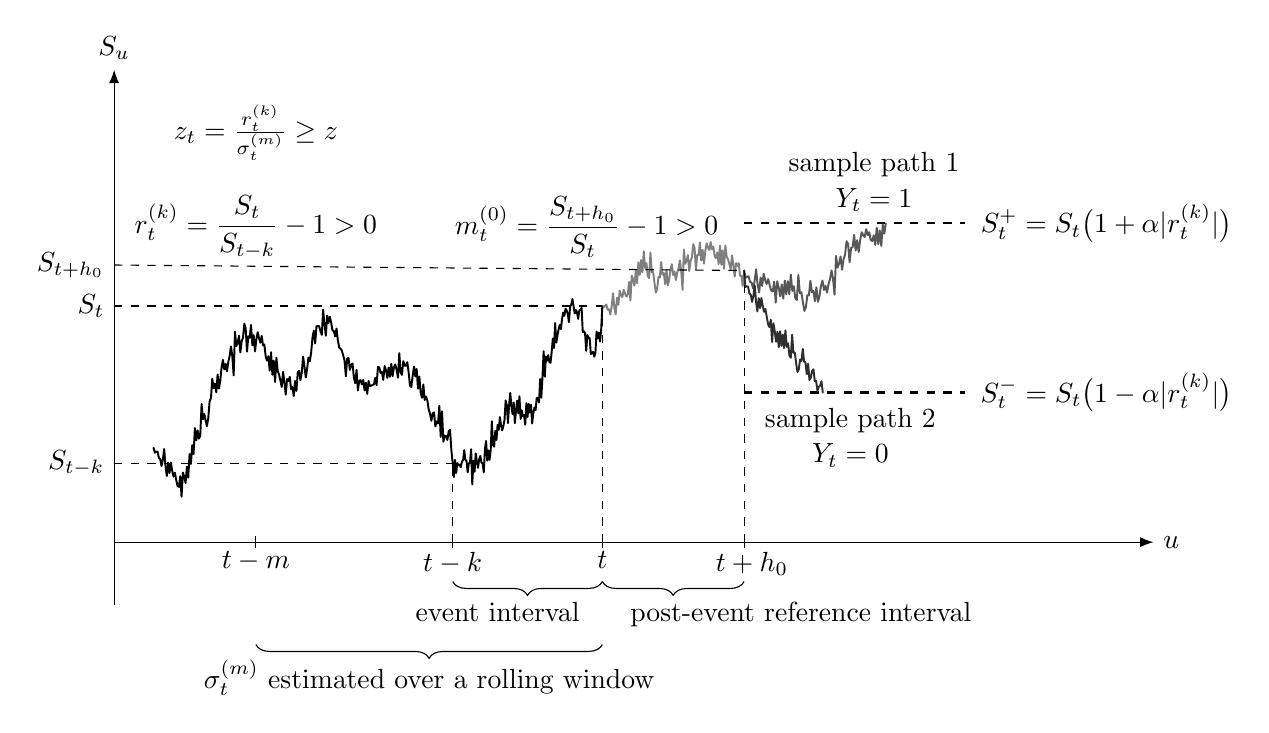
\begin{tikzpicture}[x=1cm,y=1cm,>=Latex]
			
			% =========================================================
			% AXES / KEY POINTS
			% =========================================================
			\draw[->] (0,0) -- (13.2,0) node[right] {$u$};
			\draw[->] (0,-0.8) -- (0,6.0) node[above] {$S_u$};
			
			\pgfmathsetmacro{\xTm}{1.8}
			\pgfmathsetmacro{\xTk}{4.3}
			\pgfmathsetmacro{\xT}{6.2}
			\pgfmathsetmacro{\xH}{8.0}      % t+h_0
			
			\pgfmathsetmacro{\yTk}{1.00}
			\pgfmathsetmacro{\yT}{3.00}
			
			\pgfmathsetmacro{\yTop}{4.05}
			\pgfmathsetmacro{\yBot}{1.90}
			
			% ticks
			\draw (\xTm,0.08) -- (\xTm,-0.08);
			\draw (\xTk,0.08) -- (\xTk,-0.08);
			\draw (\xT,0.08) -- (\xT,-0.08);
			\draw (\xH,0.08) -- (\xH,-0.08);
			
			\node[below] at (\xTm,0) {$t-m$};
			\node[below] at (\xTk,0) {$t-k$};
			\node[below] at (\xT,0) {$t$};
			\node[below] at (8.1,0) {$t+h_0$};
			
			
			
			% braces
			\draw[decorate,decoration={brace,mirror,amplitude=5pt}]
			(\xTm,-1.3) -- (\xT,-1.3)
			node[midway,below=2pt,align=center]
			{$\sigma_t^{(m)}$ estimated over a rolling window};
			
			\draw[decorate,decoration={brace,mirror,amplitude=5pt}]
			(\xTk,-0.5) -- (\xT,-0.5)
			node[midway,below=4pt, pos = 0.3] {event interval};
			
			\draw[decorate,decoration={brace,mirror,amplitude=5pt}]
			(\xT,-0.5) -- (\xH,-0.5)
			node[midway,below=4pt, align=center, pos = 1.4]
			{post-event reference interval};
			
			% formulas
			\node[align=left] at (1.8,4)
			{$r_t^{(k)}=\dfrac{S_t}{S_{t-k}}-1>0$};
			
			\node [align = left] at (1.8,5.2) 
			{$z_t=\frac{r_t^{(k)}}{\sigma_t^{(m)}}\ge z$};
			
			\node at (6,4)
			{$m_t^{(0)}=\dfrac{S_{t+h_0}}{S_t}-1>0$};
			
			% barrier levels
			\draw[dashed, thick] (\xH,\yTop) -- (10.8,\yTop);
			\draw[dashed, thick] (\xH,\yBot) -- (10.8,\yBot);
			
			\node at (12.6,\yTop)
			{$S_t^{+}=S_t\bigl(1+\alpha |r_t^{(k)}|\bigr)$};
			
			\node at (12.6,\yBot)
			{$S_t^{-}=S_t\bigl(1-\alpha |r_t^{(k)}|\bigr)$};
			
			% =========================================================
			% 1) GRAY PRE-EVENT PATH  [xA, xT]
			% =========================================================
			\pgfmathsetseed{9}
			
			\def\graycoords{}
			
			\pgfmathsetmacro{\xA}{0.5}
			\pgfmathsetmacro{\xMid}{6.00}
			\pgfmathsetmacro{\xBgray}{\xT}
			
			\pgfmathsetmacro{\yA}{1.20}
			\pgfmathsetmacro{\yBgray}{\yT}
			
			\pgfmathtruncatemacro{\NgrayA}{224}
			\pgfmathtruncatemacro{\NgrayB}{130}
			
			% event-interval pulls
			\pgfmathsetmacro{\cEventOne}{5}
			\pgfmathsetmacro{\aEventOne}{17}
			\pgfmathsetmacro{\wEventOne}{0.25}
			
			\pgfmathsetmacro{\cEventTwo}{5.8}
			\pgfmathsetmacro{\aEventTwo}{60}
			\pgfmathsetmacro{\wEventTwo}{0.43}
			
			% broad pulls
			\pgfmathsetmacro{\cOne}{0.85}
			\pgfmathsetmacro{\aOne}{-8}
			\pgfmathsetmacro{\wOne}{0.2}
			
			\pgfmathsetmacro{\cTwo}{1.7}
			\pgfmathsetmacro{\aTwo}{22}
			\pgfmathsetmacro{\wTwo}{0.53}
			
			\pgfmathsetmacro{\cThree}{2.7}
			\pgfmathsetmacro{\aThree}{24}
			\pgfmathsetmacro{\wThree}{0.36}
			
			\pgfmathsetmacro{\cFour}{3.6}
			\pgfmathsetmacro{\aFour}{16}
			\pgfmathsetmacro{\wFour}{0.5}
			
			\pgfmathsetmacro{\noiseLevel}{0.1}
			\pgfmathsetmacro{\pullLevel}{0.065}
			\pgfmathsetmacro{\baseLevel}{1.00}
			
			\pgfmathsetmacro{\y}{\yA}
			\xdef\graycoords{(\xA,\yA)}
			
			\foreach \i in {1,...,\NgrayA}{
				\pgfmathsetmacro{\x}{\xA + (\xTk-\xA)*\i/\NgrayA}
				\pgfmathsetmacro{\xi}{rnd+rnd+rnd+rnd+rnd+rnd+rnd+rnd+rnd+rnd+rnd+rnd-6}
				
				\pgfmathsetmacro{\shape}{
					\baseLevel
					+ \aOne   * exp(-((\x-\cOne)^2)   / (\wOne*\wOne))
					+ \aTwo   * exp(-((\x-\cTwo)^2)   / (\wTwo*\wTwo))
					+ \aThree * exp(-((\x-\cThree)^2) / (\wThree*\wThree))
					+ \aFour  * exp(-((\x-\cFour)^2)  / (\wFour*\wFour))
				}
				
				\pgfmathsetmacro{\y}{\y + \noiseLevel*\xi + \pullLevel*(\shape-\y)}
				
				\ifnum\i=\NgrayA
				\pgfmathsetmacro{\y}{\yTk}
				\fi
				
				\xdef\graycoords{\graycoords (\x,\y)}
			}
			
			\pgfmathsetmacro{\y}{\yTk}
			\pgfmathsetmacro{\tauMid}{(\xMid-\xTk)/(\xBgray-\xTk)}
			
			\foreach \i in {1,...,\NgrayB}{
				\pgfmathsetmacro{\tau}{\i/\NgrayB}
				\pgfmathsetmacro{\x}{\xTk + (\xBgray-\xTk)*\tau}
				\pgfmathsetmacro{\xi}{rnd+rnd+rnd+rnd+rnd+rnd+rnd+rnd+rnd+rnd+rnd+rnd-6}
				\pgfmathsetmacro{\theta}{max(0,(\tau-\tauMid)/(1-\tauMid))}
				
				\pgfmathsetmacro{\target}{
					\yTk
					+ (\yBgray-\yTk)*(\theta^1.8)
					+ \aEventOne * exp(-((\x-\cEventOne)^2)/(\wEventOne*\wEventOne))
					+ \aEventTwo * exp(-((\x-\cEventTwo)^2)/(\wEventTwo*\wEventTwo))
				}
				
				\pgfmathsetmacro{\noise}{0.12 - 0.033*\theta}
				\pgfmathsetmacro{\pull}{0.033 + 0.03*\theta^2}
				
				\pgfmathsetmacro{\y}{\y + \noise*\xi + \pull*(\target-\y)}
				
				\ifnum\i=\NgrayB
				\pgfmathsetmacro{\y}{\yBgray}
				\fi
				
				\xdef\graycoords{\graycoords (\x,\y)}
			}
			
			\draw[line width=0.7pt, line join=round, line cap=round]
			plot coordinates {\graycoords};
			
			% =========================================================
			% 2) Cyan PATH ON [t, t+h0]  (positive post-sign branch only)
			% tweak cCyan*, aCyan*, wCyan*, noiseCyan, pullCyan
			% =========================================================
			\pgfmathsetseed{9}
			
			\def\cyancoords{}
			\pgfmathsetmacro{\xCyanA}{\xT}
			\pgfmathsetmacro{\xCyanB}{\xH}
			\pgfmathsetmacro{\yCyanA}{\yT}
			\pgfmathsetmacro{\yCyanB}{3.45}
			\pgfmathtruncatemacro{\NCyan}{106}
			
			\pgfmathsetmacro{\cCyanOne}{6.7}
			\pgfmathsetmacro{\aCyanOne}{12}
			\pgfmathsetmacro{\wCyanOne}{0.2}
			
			\pgfmathsetmacro{\cCyanTwo}{7.5}
			\pgfmathsetmacro{\aCyanTwo}{20 }
			\pgfmathsetmacro{\wCyanTwo}{0.6}
			
			\pgfmathsetmacro{\noiseCyan}{0.1}
			\pgfmathsetmacro{\pullCyan}{0.007}
			
			\pgfmathsetmacro{\y}{\yCyanA}
			\xdef\cyancoords{(\xCyanA,\yCyanA)}
			
			\foreach \i in {1,...,\NCyan}{
				\pgfmathsetmacro{\tau}{\i/\NCyan}
				\pgfmathsetmacro{\x}{\xCyanA + (\xCyanB-\xCyanA)*\tau}
				\pgfmathsetmacro{\xi}{rnd+rnd+rnd+rnd+rnd+rnd+rnd+rnd+rnd+rnd+rnd+rnd-6}
				
				\pgfmathsetmacro{\target}{
					\yCyanA + (\yCyanB-\yCyanA)*(\tau^1.35)
					+ \aCyanOne * exp(-((\x-\cCyanOne)^2)/(\wCyanOne*\wCyanOne))
					+ \aCyanTwo * exp(-((\x-\cCyanTwo)^2)/(\wCyanTwo*\wCyanTwo))
				}
				
				\pgfmathsetmacro{\noise}{\noiseCyan - 0.01*\tau}
				\pgfmathsetmacro{\pull}{0.03 + \pullCyan*\tau^2}
				
				\pgfmathsetmacro{\y}{\y + \noise*\xi + \pull*(\target-\y)}
				
				\ifnum\i=\NCyan
				\pgfmathsetmacro{\y}{\yCyanB}
				\fi
				
				\xdef\cyancoords{\cyancoords (\x,\y)}
			}
			
			\draw[gray, line width=0.7pt, line join=round, line cap=round]
			plot coordinates {\cyancoords};
			
			% =========================================================
			% 3) PINK CONTINUATION PATH  [t+h0, ...]
			% tweak cPink*, aPink*, wPink*, noisePink, pullPink
			% =========================================================
			\pgfmathsetseed{9}
			
			\def\pinkcoords{}
			\pgfmathsetmacro{\xPzero}{\xH}
			\pgfmathsetmacro{\xPone}{9.8}
			\pgfmathsetmacro{\yPzero}{\yCyanB}
			\pgfmathsetmacro{\yPone}{\yTop}
			\pgfmathtruncatemacro{\NPink}{94}
			
			\pgfmathsetmacro{\cPinkOne}{8.4}
			\pgfmathsetmacro{\aPinkOne}{-9}
			\pgfmathsetmacro{\wPinkOne}{0.4}
			
			\pgfmathsetmacro{\cPinkTwo}{8.9}
			\pgfmathsetmacro{\aPinkTwo}{-8}
			\pgfmathsetmacro{\wPinkTwo}{0.3}
			
			\pgfmathsetmacro{\cPinkThree}{9.3}
			\pgfmathsetmacro{\aPinkThree}{4}
			\pgfmathsetmacro{\wPinkThree}{0.8}
			
			\pgfmathsetmacro{\noisePink}{0.1}
			\pgfmathsetmacro{\pullPink}{0.11}
			
			\pgfmathsetmacro{\y}{\yPzero}
			\xdef\pinkcoords{(\xPzero,\yPzero)}
			
			\foreach \i in {1,...,\NPink}{
				\pgfmathsetmacro{\tau}{\i/\NPink}
				\pgfmathsetmacro{\x}{\xPzero + (\xPone-\xPzero)*\tau}
				\pgfmathsetmacro{\xi}{rnd+rnd+rnd+rnd+rnd+rnd+rnd+rnd+rnd+rnd+rnd+rnd-6}
				
				\pgfmathsetmacro{\target}{
					\yPzero + (\yPone-\yPzero)*(\tau^1.9)
					+ \aPinkOne   * exp(-((\x-\cPinkOne)^2)   / (\wPinkOne*\wPinkOne))
					+ \aPinkTwo   * exp(-((\x-\cPinkTwo)^2)   / (\wPinkTwo*\wPinkTwo))
					+ \aPinkThree * exp(-((\x-\cPinkThree)^2) / (\wPinkThree*\wPinkThree))
				}
				
				\pgfmathsetmacro{\noise}{\noisePink - 0.02*\tau}
				\pgfmathsetmacro{\pull}{0.02 + \pullPink*\tau^2}
				
				\pgfmathsetmacro{\y}{\y + \noise*\xi + \pull*(\target-\y)}
				
				\ifnum\i=\NPink
				\pgfmathsetmacro{\y}{\yPone}
				\fi
				
				\xdef\pinkcoords{\pinkcoords (\x,\y)}
			}
			
			\draw[black!66, line width=0.7pt, line join=round, line cap=round]
			plot coordinates {\pinkcoords};
			
			% =========================================================
			% 4) GREEN REVERSAL PATH  [t+h0, ...]
			% tweak cGreen*, aGreen*, wGreen*, noiseGreen, pullGreen
			% =========================================================
			\pgfmathsetseed{9}
			
			\def\greencoords{}
			\pgfmathsetmacro{\xGzero}{\xH}
			\pgfmathsetmacro{\xGone}{9}
			\pgfmathsetmacro{\yGzero}{\yCyanB}
			\pgfmathsetmacro{\yGone}{\yBot}
			\pgfmathtruncatemacro{\NGreen}{59}
			
			\pgfmathsetmacro{\cGreenOne}{8.2}
			\pgfmathsetmacro{\aGreenOne}{-4}
			\pgfmathsetmacro{\wGreenOne}{0.20}
			
			\pgfmathsetmacro{\cGreenTwo}{8.4}
			\pgfmathsetmacro{\aGreenTwo}{-5}
			\pgfmathsetmacro{\wGreenTwo}{0.22}
			
			\pgfmathsetmacro{\cGreenThree}{8.58}
			\pgfmathsetmacro{\aGreenThree}{-10}
			\pgfmathsetmacro{\wGreenThree}{0.7}
			
			\pgfmathsetmacro{\noiseGreen}{0.1}
			\pgfmathsetmacro{\pullGreen}{0.15}
			
			\pgfmathsetmacro{\y}{\yGzero}
			\xdef\greencoords{(\xGzero,\yGzero)}
			
			\foreach \i in {1,...,\NGreen}{
				\pgfmathsetmacro{\tau}{\i/\NGreen}
				\pgfmathsetmacro{\x}{\xGzero + (\xGone-\xGzero)*\tau}
				\pgfmathsetmacro{\xi}{rnd+rnd+rnd+rnd+rnd+rnd+rnd+rnd+rnd+rnd+rnd+rnd-6}
				
				\pgfmathsetmacro{\target}{
					\yGzero + (\yGone-\yGzero)*(\tau^1.55)
					+ \aGreenOne   * exp(-((\x-\cGreenOne)^2)   / (\wGreenOne*\wGreenOne))
					+ \aGreenTwo   * exp(-((\x-\cGreenTwo)^2)   / (\wGreenTwo*\wGreenTwo))
					+ \aGreenThree * exp(-((\x-\cGreenThree)^2) / (\wGreenThree*\wGreenThree))
				}
				
				\pgfmathsetmacro{\noise}{\noiseGreen - 0.02*\tau}
				\pgfmathsetmacro{\pull}{0.025 + \pullGreen*\tau^2}
				
				\pgfmathsetmacro{\y}{\y + \noise*\xi + \pull*(\target-\y)}
				
				\ifnum\i=\NGreen
				\pgfmathsetmacro{\y}{\yGone}
				\fi
				
				\xdef\greencoords{\greencoords (\x,\y)}
			}
			
			\draw[black!82, line width=0.7pt, line join=round, line cap=round]
			plot coordinates {\greencoords};
			
			% labels
			\node at (9.65,4.8) {sample path 1};
			\node at (9.65,4.35) {$Y_t=1$};
			
			\node at (9.35,1.55) {sample path 2};
			\node at (9.35,1.10) {$Y_t=0$};
			
			% guides
			\draw[dashed] (\xTk,0) -- (\xTk,\yTk);
			\draw[dashed] (\xT,0) -- (\xT,\yT);
			\draw[dashed] (\xH,0) -- (\xH,3.45);
			
			\draw[dashed] (0,\yT) -- (\xT,\yT);
			\draw[dashed] (0,\yTk) -- (\xTk,\yTk);
			\draw[dashed] (0,3.52) -- (\xH,3.45);
			
			\node[left] at (0,3.52) {$S_{t+h_0}$};
			\node[left] at (0,\yT) {$S_t$};
			\node[left] at (0,\yTk) {$S_{t-k}$};
			
		\end{tikzpicture}
		\caption{Illustration of Method II for an upward event with \(m_t^{(0)}>0\). The event is detected at time \(t\) using the same rule as in Method I. The short post-event move over \([t,t+h_0]\) establishes a positive reference direction. Continuation \((Y_t=1)\) corresponds to the upper barrier \(S_t^{+}=S_t(1+\alpha |r_t^{(k)}|)\) being hit first, while reversal \((Y_t=0)\) corresponds to the lower barrier \(S_t^{-}=S_t(1-\alpha |r_t^{(k)}|)\) being hit first.}
		\label{fig:method2_positive_post_sign}
	\end{figure}
	
	\subsection{Conceptual Difference Between the Two Targets}
	
	The substantive difference between the two methods is not merely that they use different reference directions, but that Method II introduces a short confirmation step before the reference direction is fixed.
	
	In Method I, the label is defined relative to the direction of the extreme event itself. Hence the target asks whether the first barrier hit after time \(t\) lies in the same direction as the original event or in the opposite direction.
	
	In Method II, the label is defined relative to the immediate post-event move over \([t,t+h_0]\). Thus the target asks whether the first barrier hit after \(h_0\) lies in the same direction as this short post-event move or in the opposite direction.
	
	This distinction has two consequences. First, the waiting step in Method II can induce a stronger marginal continuation bias, since the short delay acts as a confirmation step: the reference direction is fixed only after the move over \([t,t+h_0]\) has been observed. Continuation is therefore measured relative to a direction that has already been partially realized, which can mechanically increase the base-rate tendency toward continuation. Second, this same construction introduces temporal separation between the pre-event feature vector \(X_t\) and the effective reference point of the label. In Method I, the label is anchored directly to the event at time \(t\); in Method II, it is anchored only after the short post-event interval. Consequently, Method II may exhibit stronger unconditional directional structure while at the same time being less predictable from pre-event features.
	
	Formally, even with the raw data, event-detection rule, and feature map held fixed, changing the target rule changes the effective sample
	\[
	\{(X_t,Y_t)\}_{t \in \mathcal{T}_{\mathrm{event}}},
	\]
	and therefore may change the sample size, the class balance, the time-to-resolution distribution, and the measured out-of-sample performance.
	
	The comparison is therefore best interpreted as a study of how target construction affects the bias--predictability tradeoff. Method I uses an immediately anchored target with weaker marginal asymmetry but greater scope for conditional prediction from \(X_t\). Method II uses a short delayed reference that strengthens the base-rate tendency toward continuation, but appears to attenuate the predictive relevance of the common pre-event feature set.
	
	\section{Feature Set and Modeling Setup}
	
	\subsection{Pre-Event Feature Construction}
	
	For each retained event time \(t \in \mathcal{T}_{\mathrm{event}}\), the model input is a feature vector
	\[
	X_t \in \mathbb{R}^p
	\]
	constructed exclusively from information available at or before time \(t\). Hence the empirical design avoids forward-looking features by construction. The feature set includes four broad groups.
	
	First, return- and volatility-based quantities:
	\[
	r_t^{(k)},\quad \sigma_t^{(m)},\quad z_t,\quad r_t^{(2)},\quad r_t^{(3)},\quad r_{t-1}^{(1)},\quad r_{t-2}^{(1)},\quad r_{t-3}^{(1)},
	\]
 	together with short rolling summaries such as
	\[
	\overline r_{t,3}^{(1)},\qquad \operatorname{sd}_{t,3}\!\left(r^{(1)}\right),\qquad \max_{j=0,1,2} r_{t-j}^{(1)},\qquad \min_{j=0,1,2} r_{t-j}^{(1)}.
	\]
	
	Second, volume- and activity-based quantities:
	\[
	\text{vol\_k\_rel},\qquad \text{vol\_1\_rel},\qquad \text{vol\_mean\_3\_rel},\qquad \text{vol\_regime}.
	\]
	
	Third, range- and candlestick-style quantities:
	\[
	\text{range\_k},\qquad \text{body},\qquad \text{bar\_range},\qquad \text{upper\_wick},\qquad \text{lower\_wick}.
	\]
	
	Fourth, short-horizon directional-composition and timing variables:
	\[
	\text{up\_frac\_3},\qquad \text{down\_frac\_3},\qquad \text{prev\_ret\_k},\qquad \text{mins\_from\_open}.
	\]
	
	The exact feature list used in the baseline model is:
	\[
	\begin{aligned}
		\{&\texttt{ret\_k},\texttt{sigma\_k},\texttt{event\_zscore},\texttt{event\_size},\texttt{vol\_k\_rel},\texttt{range\_k},\texttt{vol\_regime},\texttt{prev\_ret\_k},\\
		&\texttt{mins\_from\_open},\texttt{ret\_2},\texttt{ret\_3},\texttt{ret\_1\_lag1},\texttt{ret\_1\_lag2},\texttt{ret\_1\_lag3},\texttt{ret\_1\_mean\_3},\\
		&\texttt{ret\_1\_std\_3},\texttt{up\_frac\_3},\texttt{down\_frac\_3},\texttt{max\_ret\_1\_3},\texttt{min\_ret\_1\_3},\texttt{body},\texttt{bar\_range},\\
		&\texttt{upper\_wick},\texttt{lower\_wick},\texttt{vol\_1\_rel},\texttt{vol\_mean\_3\_rel}\}.
	\end{aligned}
	\]
	
	No post-event quantities used in the target construction are included as predictors. In particular, variables such as the post-event sign, hit time, hit move, or other path-dependent outcome quantities are excluded from \(X_t\).
	
	\subsection{Train-Test Split and Baseline Model}
	
	Let
	\[
	\{(X_t,Y_t)\}_{t=1}^{N}
	\]
	denote the event-level dataset ordered chronologically by event time. To preserve temporal ordering, the sample is split into a training block and a test block using a chronological \(70/30\) split:
	\[
	\{1,\dots,\lfloor 0.7N \rfloor\}
	\quad \text{for training,}
	\qquad
	\{\lfloor 0.7N \rfloor +1,\dots,N\}
	\quad \text{for testing.}
	\]
	
	The baseline classifier is logistic regression applied after feature standardization. Thus the fitted model is
	\[
	\mathbb{P}(Y_t=1\mid X_t)
	=
	\frac{1}{1+\exp\!\left(-(\beta_0+\beta^\top \widetilde X_t)\right)},
	\]
	where \(\widetilde X_t\) denotes the standardized feature vector. In implementation terms, the estimation pipeline is 
	\[
	X_t \xrightarrow{\text{StandardScaler}} \widetilde X_t \xrightarrow{\text{LogisticRegression}} \widehat Y_t
	\]
	
	\[
	\widetilde X_{t,j}=\frac{X_{t,j}-\mu_j}{s_j}
	\]
	where \(\mu_j\) and \({s_j}\) are computed from the training set, and then logistic regression is fit using \(\widetilde X_{t,j}\).
	
	This baseline was chosen deliberately. The purpose is not to maximize predictive performance, but to provide a transparent linear benchmark against which the sensitivity of the target construction can be evaluated.
	
	As a trivial comparator, a majority-class baseline is also reported. Let
	\[
	\widehat y_{\mathrm{base}}
	=
	\operatorname{mode}\{Y_t : t \in \text{training set}\}.
	\]
	The baseline classifier then predicts this same class for every observation in the test set.
	
	\subsection{Evaluation Metrics}
	
	Model performance is evaluated on the test block using accuracy, the majority-class baseline, the confusion matrix, the classification report, and ROC-AUC.
	
	The test accuracy is
	\[
	\operatorname{Acc}
	=
	\frac{1}{N_{\mathrm{test}}}
	\sum_{t \in \mathcal{T}_{\mathrm{test}}}
	\mathbf{1}\{\widehat Y_t = Y_t\}.
	\]
	Since some target constructions may produce substantial class imbalance, this quantity is reported together with the majority-class baseline
	\[
	\operatorname{Acc}_{\mathrm{base}}
	=
	\max\!\left\{
	\frac{1}{N_{\mathrm{test}}}\sum_{t\in\mathcal{T}_{\mathrm{test}}}\mathbf{1}\{Y_t=0\},
	\;
	\frac{1}{N_{\mathrm{test}}}\sum_{t\in\mathcal{T}_{\mathrm{test}}}\mathbf{1}\{Y_t=1\}
	\right\},
	\]
	
	This comparator is substantively important in the present setting. A target construction may induce strong class imbalance and therefore high unconditional predictability in the trivial sense that one class occurs much more often than the other. Outperforming the majority baseline is therefore interpreted as evidence of conditional predictive structure beyond the marginal class distribution.
	
	To describe the composition of correct and incorrect predictions, the confusion matrix is reported:
	\[
	C
	=
	\begin{pmatrix}
		C_{00} & C_{01}\\
		C_{10} & C_{11}
	\end{pmatrix},
	\qquad
	C_{ij}
	=
	\#\{t \in \mathcal{T}_{\mathrm{test}} : Y_t=i,\ \widehat Y_t=j\}.
	\]
	Thus
	\[
	C_{00}=\text{true negatives},\qquad
	C_{01}=\text{false positives},\qquad
	C_{10}=\text{false negatives},\qquad
	C_{11}=\text{true positives}.
	\]
	The confusion matrix is useful because two models with similar accuracy may behave very differently across the two classes. In particular, under class imbalance, a classifier may achieve high raw accuracy simply by overpredicting the majority class.
	
	The classification report summarizes precision, recall, and \(F_1\)-score. For class \(1\),
	\[
	\operatorname{Precision}_1
	=
	\frac{C_{11}}{C_{01}+C_{11}},
	\qquad
	\operatorname{Recall}_1
	=
	\frac{C_{11}}{C_{10}+C_{11}},
	\]
	and
	\[
	F_{1,1}
	=
	\frac{2\,\operatorname{Precision}_1\,\operatorname{Recall}_1}
	{\operatorname{Precision}_1+\operatorname{Recall}_1}.
	\]
	Analogous definitions apply to class \(0\).
	
	Let
	\[
	\widehat p_t = \mathbb{P}(Y_t=1\mid X_t)
	\]
	denote the fitted logistic probability. ROC-AUC is computed from the receiver operating characteristic curve obtained by varying the classification threshold \(c \in [0,1]\). For each threshold \(c\), define
	\[
	\widehat Y_t(c)=\mathbf{1}\{\widehat p_t \ge c\}.
	\]
	This yields the true positive rate
	\[
	\operatorname{TPR}(c)
	=
	\frac{\#\{t:Y_t=1,\ \widehat Y_t(c)=1\}}
	{\#\{t:Y_t=1\}},
	\]
	and the false positive rate
	\[
	\operatorname{FPR}(c)
	=
	\frac{\#\{t:Y_t=0,\ \widehat Y_t(c)=1\}}
	{\#\{t:Y_t=0\}}.
	\]
	The ROC curve is the set
	\[
	\{(\operatorname{FPR}(c),\operatorname{TPR}(c)) : c\in[0,1]\},
	\]
	and the area under this curve is the ROC-AUC:
	\[
	\operatorname{AUC}
	=
	\int_0^1 \operatorname{TPR}(u)\,d u,
	\]
	where \(u\) denotes the false positive rate parametrizing the curve.
	
	Equivalently, ROC-AUC admits the probabilistic interpretation
	\[
	\operatorname{AUC}
	=
	\mathbb{P}\!\left(\widehat p_i > \widehat p_j \mid Y_i=1,\ Y_j=0\right),
	\]
	up to ties. Hence ROC-AUC measures ranking quality: it is the probability that a randomly chosen positive observation receives a higher model score than a randomly chosen negative observation.
	
	This metric is particularly useful here because a model may achieve moderate accuracy simply by tracking the dominant class, whereas ROC-AUC evaluates whether the fitted probabilities actually separate continuation from reversal. In particular,
	\[
	\operatorname{AUC}\approx 0.5
	\]
	indicates no meaningful discrimination, even if raw accuracy appears acceptable, while
	\[
	\operatorname{AUC}>0.5
	\]
	indicates that the model contains some ranking information beyond chance.
	
	\section{Empirical Results}
	
	\subsection{Dataset Size and Marginal Label Distribution}
	
	Under the common event-detection backbone and the common pre-event feature set, the two target constructions produce materially different event-level datasets.
	
	For Method I (event-direction reference), the final labelled sample contains
	\[
	N = 201
	\]
	events, with empirical continuation rate
	\[
	\widehat{\mathbb{P}}(Y=1)=0.478.
	\]
	Thus the induced target is close to balanced.
	
	For Method II (post-event / next-bar reference), the final labelled sample contains
	\[
	N = 165
	\]
	events, with empirical continuation rate
	\[
	\widehat{\mathbb{P}}(Y=1)=0.703.
	\]
	Hence the delayed reference construction induces a substantially stronger skew toward continuation.
	
	This difference is itself substantive. The short waiting step in Method II fixes the reference direction only after the move over \([t,t+h_0]\) has been observed. As a result, continuation is measured relative to a direction that has already been partially realized, which mechanically increases the marginal tendency toward continuation. Thus the first effect of target construction is distributional:
	\[
	\text{Method I} \;\Rightarrow\; \text{near-balanced labels},
	\qquad
	\text{Method II} \;\Rightarrow\; \text{continuation-dominated labels}.
	\]
	
	\subsection{Out-of-Sample Predictive Performance}
	
	The out-of-sample results differ sharply across the two specifications.
	
	For Method I, the chronological test-set accuracy is
	\[
	\mathrm{Acc}=0.623,
	\]
	while the majority-class baseline is
	\[
	\mathrm{Acc}_{\mathrm{base}}=0.492.
	\]
	The corresponding ROC-AUC is
	\[
	\mathrm{AUC}=0.591.
	\]
	Thus Method I exhibits modest but nontrivial predictive discrimination beyond the marginal class distribution.
	
	For Method II, the test-set accuracy is
	\[
	\mathrm{Acc}=0.720,
	\]
	but the majority-class baseline is even higher:
	\[
	\mathrm{Acc}_{\mathrm{base}}=0.760.
	\]
	Moreover, the ROC-AUC is
	\[
	\mathrm{AUC}=0.471,
	\]
	which lies below random ranking. Hence the apparent raw accuracy of Method II is driven primarily by the strong continuation skew in the target rather than by useful conditional prediction from \(X_t\).
	
	Accordingly, the main empirical contrast is not that one specification attains higher headline accuracy than the other, but that they differ in the relation between marginal bias and conditional learnability:
	\[
	\text{Method I: weaker marginal bias, stronger conditional predictability;}
	\]
	\[
	\text{Method II: stronger marginal bias, weaker conditional predictability.}
	\]
	
	\subsection{Confusion-Matrix Comparison}
	
	The test-set confusion matrix for Method I is
	\[
	C^{(I)}=
	\begin{pmatrix}
		20 & 10\\
		13 & 18
	\end{pmatrix}.
	\]
	This matrix is reasonably balanced across the two classes. The classifier identifies both continuation and reversal with comparable success, which is consistent with the near-symmetric label distribution and the ROC-AUC above \(0.5\).
	
	For Method II, the confusion matrix is
	\[
	C^{(II)}=
	\begin{pmatrix}
		1 & 11\\
		3 & 35
	\end{pmatrix}.
	\]
	This matrix is highly asymmetric. In particular, the classifier correctly identifies only \(1\) out of \(12\) reversal events in the test set, while correctly classifying most continuation events. Thus the model is effectively overpredicting continuation, which explains why its raw accuracy remains moderate despite weak ranking quality.
	
	The confusion matrices therefore reinforce the same conclusion: Method II produces a target with stronger class asymmetry, but the fitted model does not extract useful class-specific discrimination beyond that asymmetry.
	
	\subsection{Interpretation}
	
	Taken together, the results support the central claim of the paper: under a fixed event-detection rule and a fixed pre-event feature set, target construction materially changes both the marginal label distribution and the apparent learnability of the prediction problem.
	
	Method II induces a pronounced unconditional continuation tendency,
	\[
	\widehat{\mathbb{P}}(Y=1)\approx 0.70,
	\]
	which is economically and statistically meaningful at the level of the marginal distribution. However, this stronger directional bias does not translate into stronger conditional prediction from pre-event features. Rather, once the majority-class effect is taken into account, Method II exhibits weak discriminatory power.
	
	Method I behaves differently. Its target distribution is much closer to balanced, yet the logistic baseline outperforms the majority classifier and achieves ROC-AUC above \(0.5\). This suggests that the event-direction target retains at least modest conditional structure that is detectable from pre-event information.
	
	A natural interpretation is that Method II trades conditional learnability for directional confirmation. By waiting one bar before fixing the reference direction, it establishes a stronger base-rate tendency toward continuation, but at the same time introduces temporal displacement between the feature vector \(X_t\) and the effective anchor of the label. Even though this displacement is small, the results suggest that it is sufficient to attenuate the predictive relevance of the common pre-event feature set.
	
	The main conclusion is therefore comparative rather than prescriptive. The strongest finding is not a robust predictive edge, but that the apparent predictability of continuation versus reversal is highly sensitive to how the target is defined. In the present setting, delayed reference construction primarily alters the base rate, whereas immediate event-direction reference preserves more conditional predictability from \(X_t\).
	
	\section{Discussion}
	
	The empirical comparison indicates that target construction affects the problem along two distinct dimensions: the marginal distribution of the label and the extent of conditional predictability from the common pre-event feature set.
	
	The first effect is distributional. Method II produces a substantially higher continuation rate than Method I. This is not incidental. In Method II, the reference direction is fixed only after the short interval \([t,t+h_0]\) has been observed. The delay therefore acts as a confirmation step: continuation is measured relative to a direction that has already been partially realized. This mechanically induces a stronger marginal bias toward continuation. By contrast, Method I anchors the label directly to the original event direction, so the induced target remains much closer to balanced.
	
	The second effect concerns learnability. Although Method II exhibits stronger unconditional directional structure, the common pre-event feature set does not predict this target more effectively than the majority-class baseline. Its higher raw accuracy is therefore not evidence of stronger conditional structure, but is largely attributable to the continuation-dominated class distribution. Method I behaves differently. Its marginal label distribution is weaker and more symmetric, yet the logistic baseline outperforms the majority classifier and attains ROC-AUC above \(0.5\). This suggests that the event-direction target preserves at least modest conditional information that is detectable from \(X_t\).
	
	These results imply that unconditional bias and conditional predictability should be distinguished carefully. A target may display strong statistical regularity at the level of
	\[
	\mathbb{P}(Y=1),
	\]
	without being especially predictable from the feature vector through
	\[
	\mathbb{P}(Y=1 \mid X_t).
	\]
	That distinction is central in the present setting. Method II appears to strengthen the former while weakening the latter. Method I, despite its weaker base-rate asymmetry, retains greater evidence of feature-based discrimination.
	
	A natural interpretation is temporal attenuation. In Method I, the feature vector \(X_t\) and the label reference point coincide at the event time \(t\). In Method II, the effective reference point is shifted forward to the end of the interval \([t,t+h_0]\). Even though \(h_0=1\) in the present implementation, this small displacement appears sufficient to weaken the alignment between the feature snapshot and the eventual label. Put differently, the missing one-bar transition may contain information that is highly relevant for the delayed-reference target but unavailable to a model restricted to pre-event inputs. Under this interpretation, the deterioration in predictive performance under Method II is not merely a consequence of changed label semantics, but of reduced temporal alignment between predictors and target.
	
	This interpretation also helps explain why the two methods may invite different feature sets. The current predictors are constructed entirely from information available at or before the event time and are therefore naturally suited to characterizing the event itself: its magnitude, local volatility context, recent return dynamics, volume conditions, and bar shape. Such quantities may be more informative for predicting whether the original event direction persists than for predicting whether a one-bar-confirmed post-event direction persists. If so, Method II may require features more closely tied to very short-horizon post-event stabilization, directional persistence, or local microstructural adjustment. In that sense, the present results do not imply that Method II is intrinsically unpredictable, only that it is not well captured by the current pre-event feature map.
	
	The results should also be interpreted in light of the data limitations. The analysis uses approximately sixty calendar days of 2-minute SPY data from \texttt{yfinance}, so the sample is short and the conclusions are necessarily exploratory. The paper therefore does not claim a stable market effect or a deployable trading rule. Rather, the evidence supports a narrower conclusion: under a fixed event-detection architecture and a fixed pre-event feature set, small changes in target construction can materially alter both the base rate of the label and the apparent success of a predictive model.
	
	From a modeling perspective, this is the main lesson. In short-horizon event-driven classification, the label is not a passive object extracted from the data, but an active design choice that helps determine what statistical structure is visible to the model. The present comparison shows that delaying the reference direction by even one bar can strengthen marginal continuation bias while attenuating conditional learnability. A natural extension is therefore to study this tradeoff more systematically. In particular, future work could investigate whether there exists an intermediate target construction that better balances directional confirmation against temporal attenuation, rather than relying only on the two endpoint specifications considered here. With a larger sample and higher-resolution intraday data, one could vary the delay used to define the reference direction and examine whether predictive performance is maximized at some intermediate labeling rule between immediate event-direction anchoring and short delayed anchoring. Access to lower time frames would be especially valuable, since finer temporal granularity would permit a more precise analysis of how feature relevance decays as the label reference point moves away from the event time. Accordingly, target construction should be treated as a first-order modeling decision rather than as a secondary implementation detail.
	
	\section{Conclusion}
	
	This paper studied continuation versus reversal after extreme short-term SPY moves under a common event-detection backbone and a common pre-event feature set, while varying only the target construction. The central finding is that the apparent predictability of the problem is materially sensitive to how the binary label is defined.
	
	When continuation and reversal are defined relative to the direction of the extreme event itself (Method I), the induced target is close to balanced and the logistic baseline exhibits modest but nontrivial predictive discrimination beyond the majority-class benchmark. When the reference direction is instead fixed only after a short post-event interval (Method II), the target becomes strongly skewed toward continuation, but this additional marginal structure does not translate into improved conditional prediction from pre-event features. In particular, the higher raw accuracy of Method II is dominated by class imbalance rather than by meaningful ranking or classification quality.
	
	The results therefore distinguish two different notions of structure. Method II exhibits stronger \emph{unconditional} directional structure, in the sense that the delayed reference construction induces a higher base-rate tendency toward continuation. Method I, by contrast, exhibits stronger \emph{conditional} structure, in the sense that the common pre-event feature set retains greater predictive relevance when the label is anchored directly to the event direction. This suggests that a short confirmation step may strengthen directional bias while simultaneously attenuating feature--label alignment.
	
	A related interpretation is temporal. In Method II, the effective reference point of the label is shifted forward relative to the feature snapshot \(X_t\). Even though this displacement is only one bar in the present implementation, the empirical results indicate that it is sufficient to weaken the extent to which the outcome can be predicted from pre-event information alone. Thus the paper identifies a bias--predictability tradeoff: waiting to confirm direction can alter the marginal distribution in a favorable directional sense, while reducing conditional learnability.
	
	The contribution is comparative rather than prescriptive. The paper does not claim a robust tradable signal. Rather, it shows that in short-horizon event-driven classification problems, target construction is not a secondary implementation detail: it changes the effective sample, the class balance, and the extent to which the label remains predictable from a fixed feature set. In the present setting, delayed reference construction primarily changes the base rate, whereas immediate event-direction reference preserves more of the conditional structure detectable from \(X_t\).
	
	A natural direction for future work is to study this tradeoff more systematically. With a larger sample and higher-resolution intraday data, one could investigate intermediate target constructions between immediate event-direction anchoring and delayed post-event anchoring, and test whether predictive performance is maximized at some more favorable balance between directional confirmation and temporal attenuation. More broadly, this type of analysis could serve as a scaffolding in the construction of a real short-horizon trading strategy: before optimizing execution or portfolio rules, one would first want to identify a target construction that preserves economically meaningful directional structure while remaining predictably linked to information available at decision time.
	
	\appendix
	
	\section{Parameter Choices}
	
	The common event-detection backbone is
	\[
	k = 3, \qquad m = 15, \qquad z = 2, \qquad \mathrm{cooldown} = 10.
	\]
	Thus an event is defined by a sufficiently large 3-bar return relative to a local 15-bar volatility scale, with at least 10 bars separating consecutive retained events.
	
	The common post-event horizon parameters are
	\[
	h_0 = 1, \qquad h_{\max} = 30, \qquad \alpha = 0.5.
	\]
	Hence, conditional on detection, the post-event path is examined for at most 30 bars, and the symmetric barrier distance is scaled by
	\[
	\alpha \lvert r_t^{(k)} \rvert.
	\]
	
	These parameters are held fixed across both target constructions. Accordingly, the empirical comparison isolates the effect of the label definition rather than changes in the event-detection rule or post-event horizon.
	
	\section{Implementation Notes}
	
	The empirical pipeline consists of four steps:
	\[
	\text{data cleaning}
	\;\longrightarrow\;
	\text{event detection}
	\;\longrightarrow\;
	\text{label construction}
	\;\longrightarrow\;
	\text{baseline classification}.
	\]
	
	Intraday SPY data are downloaded from \texttt{yfinance} and converted to a 2-minute time series. Events too close to the end of the sample are dropped when the full post-event horizon is unavailable.
	
	For both methods, the same pre-event feature set is used. Hence all differences in empirical results are attributable to the target construction rather than to differences in the predictor set.
	
	The baseline classifier is estimated through the pipeline
	\[
	X_t \xrightarrow{\text{StandardScaler}} \widetilde{X}_t \xrightarrow{\text{LogisticRegression}} \widehat{Y}_t,
	\]
	with chronological train--test splitting used to preserve temporal ordering.
	
	In addition to raw accuracy, the analysis reports the majority-class baseline, the confusion matrix, and ROC-AUC. This is important because the two target constructions induce materially different class balances. In particular, raw accuracy alone may be misleading when
	\[
	\mathbb{P}(Y=1)
	\]
	is far from \(0.5\). The majority baseline and ROC-AUC are therefore used to distinguish unconditional class skew from genuine conditional predictive discrimination.
	
\end{document}